\documentclass[a4paper]{article}
\usepackage[utf8]{inputenc}
\usepackage[english,italian]{babel}
\usepackage{afterpage}
\usepackage{graphicx}
\usepackage{fancyvrb}
\usepackage[inline]{enumitem}

\title{RELAZIONE PROGETTO\\PROGRAMMAZIONE ad OGGETTI}
\author{Nicola Dalla Costa (1051222)}
\date{}

\begin{document}
\maketitle
\raggedbottom

\renewcommand\abstractname{\textit{Abstract}}
\begin{abstract}
\noindent Lo scopo del progetto, denominato \textit{LinQedIn}, era lo sviluppo in C++/Qt di un sistema minimale per l'amministrazione ed utilizzo tramite interfaccia utente grafica di un (piccolo) database di contatti professionali ispirato a LinkedIn. 

LinkedIn è il principale servizio web di rete sociale per contatti professionali, gratuito ma con servizi opzionali a pagamento.
\end{abstract}

\section*{Introduzione}
Attualmente LinkedIn prevede quattro tipologie di account, ma per semplicità sono state considerate solo Business ed Exectutive, oltre a quella gratuita Basic.

Tra le funzionalità disponibili all'utente amministratore troviamo: inserimento e rimozione utenti, ricerca utenti e cambio tipologia di account di un utente. Lato utente invece sono disponibili: aggiornamento informazioni profilo, aggiunta e rimozione contatti, titoli di studio ed esperienze lavorative, ed una funzionalità di ricerca crescenti in base alla tipologia di account.

Per la realizzazione della GUI è stato utilizzato IDE QtCreator ma senza l'ausilio del tool QtDesigner. In questo modo il codice risulta più pulito.

Nonostante il progetto si limiti ad offrire le funzionalità richieste, nella realizzazione è stata data molta importanza a concetti come information hiding, modularità, estendibilità e qualità del codice.

La realizzazione del progetto è costata solo nell'ultimo mese di lavoro più di 100 ore. Impossibile definire una quantità totale indicativa.

La presente relazione non deve essere considerata come documentazione. Viene fornita una breve descrizione di tutte le classi e della logica, soffermandosi solo nei dettagli più importanti.\footnote{Una documentazione più dettagliata è presente nel codice sottoforma di commenti.}

\section*{Parte Logica}
La parte logica si compone di 16 classi che ora vederemo nel dettaglio. Per semplicità saranno considerati solo i metodi più importanti, mentre saranno omessi i metodi getter e setter dei campi dati.

\subsection*{Profilo}
Utilizzata per la gestione delle informazioni personali di un utente. Sono state considerate: nome, cognome, data di nascita e stato civile. 

La rappesentazione interna viene nascosta con l'utilizzo di un puntatore ad una classe interna privata InfoPersonali. In questo modo viene nascosto all'utente finale la modalità di memorizzazione dei dati (\textit{information hiding}).

L'utilizzo di un puntatore per nascondere la rappresentazione interna può provocare problemi di condivisione di memoria. Per questo motivo in caso di costruzione di copia di un oggetto Profilo, viene effettuata una copia profonda dei campi dati puntatore. In questi casi è necessario che anche l'operatore di assegnazione sia ridefinito in modo che effettui un'assegnazione profonda.

\subsection*{Rete}
Utilizzata per la gestione della lista dei contatti di un utente. I contatti sono memorizzati come oggetti di tipo SmartUtente che saranno descritti più avanti.

La rappresentazione interna viene nascosta con l'utilizzo di un puntatore ad una classe interna privata Rete\_rapp. A differenza del campo dati di tipo InfoPersonali* per il Profilo, qui si è pensato di gestire la copia di oggetti Rete con la tecnica del \textit{references counting}: in caso di copia o distruzione di un oggetto Rete si limita ad incrementare o diminuire il campo riferimenti. La distruzione effettiva si verifica solo quando il campo riferimenti arriva a 0.

Per ottenere la lista dei contatti, poichè non è nota la modalità di memorizzazione, è stato fornito il metodo \texttt{QVector<SmartUtente> getContactsList() const} che ritorna la lista dei contatti in un semplice vettore.

\subsection*{Lavoro e Titolo}
Utilizzate per la gestione delle esperienze lavorative e dei titoli di studio rispettivamente. La prima memorizza informazioni riguardo a nome azienda, ruolo ricoperta, data di inizio e fine. La seconda memorizza nome scuola o università, data di conseguimento diploma o laurea e campo di studi.

Sono inoltre fornite le due classi \textbf{SmartLavoro} e \textbf{SmartTitolo}, le quali permettono di gestire in modo automatico il campo riferimenti in caso di condivisione di memoria tra puntatori ad oggetti di tipo Lavoro o Titolo.

\subsection*{Esperienza e Formazione}
Utilizzate per memorizzare la lista delle esperienze lavorative e dei titoli di studio di un utente, memorizzati come puntatori ad oggetti Lavoro e Titolo.

Come per la classe Rete, la rappresentazione interna viene nascosta con l'utilizzo di puntatori alle classi interne private Esperienza\_rapp e Formazione\_rapp definite. La copia degli oggetti viene sempre gestita con la tecnica del references counting e sono disponibili metodi per ottenere le liste come vettori.

Per entrambe è stato inoltre fornito un iteratore con i soli metodi \texttt{begin()}, \texttt{hasNext()} e \texttt{next()}. La realizzazione di questi iteratori è stata difficile in quanto le classi interne possono accedere solo ai membri statici delle classi contenitrici ed entrambe le classi (contenitrice ed iteratore) dovevano rispettare l'information hiding.

\subsection*{Utente}
Utilizzata per la gestione dei signoli utenti del client. Contiene un campo dati di tipo QString per memorizzare l'username, un campo dati Profilo e tre campi dati puntatore ad oggetti di tipo Rete, Formazione ed Esperienza. 

La scelta dei puntatori è dovuta al fatto che le liste possono crescere e la copia di utenti potrebbe comportare spreco di memoria. La copia degli utenti viene sempre gestita con la tecnica del references counting.

Fornire metodi che permettono un accesso diretto ad un campo dati tramite puntatore non è una buona pratica. Per questo motivo sono stati riportati tutti i metodi pubblici dei campi dati puntatore nella classe Utente, i quali invocano i metodi corrispondenti nella classe di appartenenza. Purtroppo in questo modo si crea una forte dipendenza con le classi Rete, Formazione ed Esperienza ma l'utilizzo dei metodi risulta più pratica.

Viene fornita inoltre la classe \textbf{SmartUtente} per la gestione automatica del campo riferimenti in caso di copie di oggetti Utente.

\subsubsection*{Gerarchia}
La classe Utente è una classe base polimorfa ed astratta in quanto contiene il distruttore definito virtuale e puro (condizione necessaria e sufficiente ma sono presenti anche altri metodi dichiarati virtuali puri).

Inizialmente erano state create due sottoclassi (sempre astratte) UtenteGratis e UtentePagante in quanto la questa differenza può significare grandi differenze. Da UtenteGratis poi veniva derivata la classe concreta \textbf{UtenteBasic}, mentre da UtentePagante venivano derivate le classi \textbf{UtenteExecutive} ed \textbf{UtenteBusiness}. Nonostante questa fosse la gerarchia corretta, data l'assenza di nuovi campi dati o metodi definiti nelle due classi intermedie (e per semplicità), è stato deciso di rimuovere UtentePagante ed UtenteGratis e far derivare direttamente le 3 classi concrete da Utente.

\subsubsection*{Ricerca}
La funzionalità di ricerca è stata l'ultima ad essere sviluppata. Purtroppo la versione definitiva non mi ha ancora convinto.

Una delle versioni faceva uso della classe FuntoreRicerca, classe funtore, definita interna ad Utente e di un metodo \texttt{QVector<SmartUtente> searchUsers( QVector<SmartUtente> )} virtuale puro che in base alla ridefinizione nelle classi concrete ritornava un vettore di nuovi oggetti SmartUtente creati di copia dal vettore passato come parametro, ai quali venivano rimossi i campi non visualizzabili in base alla tipologia. 

Questo però aveva comportato la necessità di aggiungere dei metodi \texttt{*clone() const} e di costruttori appositi in tutte le classi concrete della gerarchia Utente e lo stesso nelle classi Rete, Formazione ed Esperienza, la ridefinizione dell'operatore \texttt{delete} nelle ultime 3 e l'aggiunta di metodi per distruggere manualmente i campi dati puntatore della classe Utente in base alle informazioni che si volevano rendere disponibili. In questo modo però era necessaria anche la modifica dei metodi della classe Utente per controllare che i campi dati puntatore fossero validi. La necessità di distruggere i campi dati era dovuta al fatto che, ad esempio, una lista di contatti vuota è diversa da una lista di contatti inaccessibile.

Anche se funzionante come soluzione era troppo complessa e c'era il forte rischio di introduzione di errori. Per questo motivo si è passati ad una soluzione molto più semplice. Tolta la classe funtore e tutti i metodi, costruttori ed operatori aggiunti, è stato aggiunto un metodo virtuale puro \texttt{QList<QString> getUserInfo() const} che restituisce una lista con degli indicatori per i campi accessibili dall'utente. Purtroppo anche se più semplice per molti versi è peggiore in quanto non ottieni direttamente le informazioni ma solo una lista dei campi accessibili.

Durante la stesura di questa relazione ho pensato come migliorare le precedenti soluzioni. La prima poteva essere migliorata già semplicemente togliendo dal costruttore di Utente la costruzione di default dei campi dati puntatore. In questo modo alla creazione dell'oggetto utente da visualizzare potevano essere aggiunti i campi desiderati. Purtroppo rimane molto complicata. Nella seconda si poteva utilizzare una mappa per restituire le informazioni ma la complessità sarebbe aumentata a causa dei valori associati alle chiavi in quanto i campi sono di tipi diversi e l'utilizzo di \texttt{void *} non sarebbe stato elegante.

\subsection*{Database}
Utilizzata per la gestione degli utenti del client. Si è deciso di memorizzare gli utenti nel database tramite una mappa, dove l'username è la chiave associata allo SmartUtente (puntatore ad Utente). La rappresentazione interna è nascosta all'utente finale tramite l'utilizzo della classe interna Database\_rapp. In questo modo il codice è indipendente dalla rappresentazione e possono essere effettuate modifiche alla modalità di memorizzazione senza aver bisogno di modificare i metodi forniti all'utente. Altro motivo è dovuto al fatto che le funzioni di ricerca, inserimento e rimozione di un utente viene fatta in tempo O(1), quindi costante.

La dichiarazione di amicizia con la classe LinQedInAdmin è necessaria in quanto i metodi, dichiarati privati, per l'inserimento e rimozione di utenti da database deve essere disponibile solo all'utente amministratore.

Il salvataggio di utenti avviene su file XML con l'utilizzo di QXmlStreamWriter, mentre il caricamento con QXmlStreamReader. In caso il file non esista viene creato. Particolare attenzione bisogna dare al caricamento degli utenti, in quanto la creazione della lista dei contatti avviene solo dopo aver caricato tutti gli utenti nel database. Questo perchè la lista dei contatti è composta da oggetti SmartUtente e non si può inserire un utente se non esiste.

\subsection*{LinQedInClient}
Utilizzata per la gesione del client lato utente. Contiente un campo dati SmartUtente che corrisponde all'utente utilizzatore del client ed un puntatore ad un oggetto Database. Mette a disposizione dei semplici metodi per salvare i campi dati dell'utente utilizzatore del client. La definizione di questi metodi si limita a richiamare la funzione \texttt{void saveUsersList() const} in quanto, essendo un piccolo database di utenti, la riscrittura di tutto il file non è onerosa.

\subsection*{LinQedInAdmin}
Utilizzata per la gestione del client lato amministratore. A differenza di LinQedInClient, questa classe funziona come controller (del pattern MVC) in quanto i metodi forniti collegano la parte logica alle funzionalità della parte grafica. Vengono messi a disposizione metodi per inserimento, rimozione, ricerca e cambio tipolgia di account degli utenti, oltre a caricamento ed salvataggio.

\section*{Parte Grafica}
La parte grafica si compone di 29 classi. Nella realizzazione della GUI si sono cercati di seguire i principi del \textit{Material Design}.

Una delle caratteristiche che accomunano tutte la componenti della GUI è la presenza dei due metodi privati ausiliari \texttt{void initUI()} e \texttt{void setupUI()} per l'inizialiazzazione e realizzazione della GUI rispettivamente. Inoltre la ridefinizione del distruttore non è necessaria in quanto nell'inizializzazione dei campi dati di tipo puntatore viene passato come QWidget parent \texttt{this}. In questo modo alla distruzione del parent (quindi dell'instaza della classe) vengono distrutti tutti gli oggetti figli.

\subsection*{LinQedInWindow}
Classe base astratta che estende QMainWindow, da utilizzare come classe base per tutte le finestre del client. Offre campi e metodi comuni. Così facendo la necessità della stessa modifica in ognuna di queste può essere effettuata una sola volta. Le classi derivate sono: LoginWindow, AdminWindow e ClientWindow.

\subsection*{LinQedInDialog}
Classe base astratta che estende QDialog, da utilizzare come classe base per tutte le finestre di dialogo del client. Come per LinQedInWindow, offre campi e metodi comuni. Le classi derivate sono: AddJobDialog, AddTitleDialog, AddUserDialog, AdminLoginDialog, AdminSearchDialog, ChangeUserTypeDialog, EditJobDialog, EditProfileDialog e EditTitleDialog.

\subsection*{LoginWindow}
\begin{figure}[!ht]
\centering
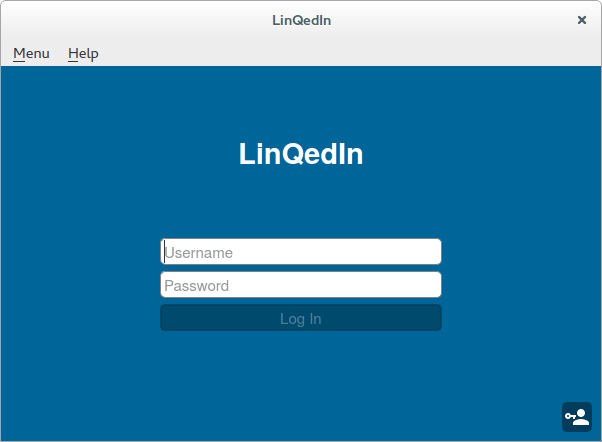
\includegraphics[width=0.6\textwidth]{LoginWindow.png}
\caption{Finestra di login}
\end{figure}

Il pulsante per l'accesso utente risulta disabilitato e viene abilitato solo quando entrabi i campi (username e password) risultano non vuoti. Per fare questo è stato connesso lo slot \texttt{void checkInput( QString )} al segnale \texttt{textChanged( QString )} che viene emesso ogni volta che il contenuto di uno tra i due oggetti QLineEdit viene modificato. Gli spazi ad inizio e fine vengono ignorati. Il controllo effettivo avviene solo nell'username, mentre il campo password è stato aggiunto solo per completezza. Il controllo di entrambi i campi non è stato ritenuto molto importante, ma è stata data più attenzione all'utilizzo corretto delle librerie Qt, alla qualità ed all'usabilità.

Al pulsante di log in è connesso lo slot \texttt{void loginUser()} che crea un'istanza di ClientWindow (passando l'username) con parent 0 (quindi top-level) e distrugge l'istanza di LoginWindow.

L'accesso amministrativo avviene tramite l'apertura della finestra di dialogo di tipo AdminLoginDialog. Alla pressione del pulsante nell'angolo in basso a destra è connesso lo slot \texttt{void openAdminLoginDialog()} che crea un oggetto \textbf{AdminLoginDialog}.

\begin{figure}[!ht]
\centering
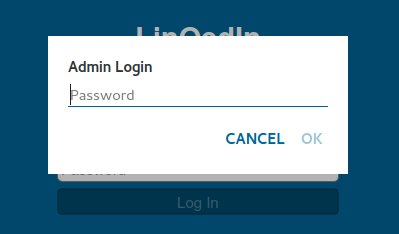
\includegraphics[width=0.4\textwidth]{AdminLoginDialog.png}
\caption{AdminLoginDialog}
\end{figure}

Nella costruzione di quest'ultima viene passato come oggetto QWidget parent l'istanza della classe LoginWindow. In questo modo non risulta possibile chiudere il client senza prima aver chiuso la finestra di dialogo.

Come per l'accesso utente, il pulsante di conferma password risulta disabilitato finchè la password inserita contiene almeno un carattere. Gli spazi ad inizio e fine sono esclusi. Al pulsante di conferma è connesso lo slot \texttt{void checkPassword()} (per semplicità, anche in questo caso non avviene una verifica effettiva) che prima chiude la finestra di login e successivamente emette il segnale \texttt{void adminLoginSignal()}. Al segnale è connesso lo slot \texttt{void adminLogin()} del parent che si comporta come lo slot per l'accesso utente ma questa volta crea un'istanza di AdminWindow.

\subsection*{ClientWindow}
Nella realizzazione della GUI della classe ClientWindow mi sono ispirato ad un concept presente su \textit{Behance}\footnote{\textit{Linkedin Material Design}, realizzato da Rico Monteiro e pubblicato con licenza ``Attribution-NonCommercial 3.0 Unported (CC BY-NC 3.0)''}.

\begin{figure}[!ht]
\centering
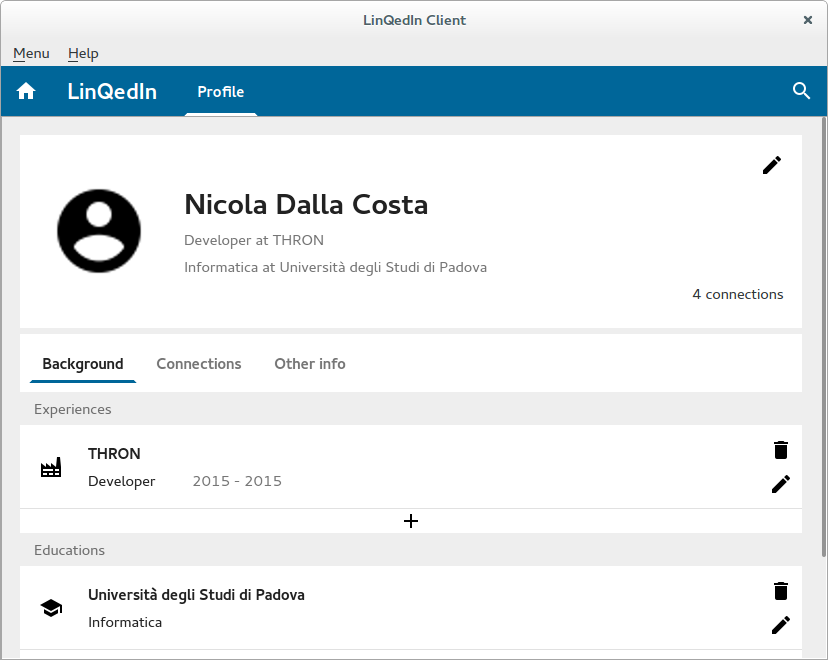
\includegraphics[width=0.6\textwidth]{ClientWindow.png}
\caption{ClientWindow}
\end{figure}

A parte i componenti grafici contiene un puntatore ad un oggetto LinQedInClient, necessario per il salvataggio delle informazioni su database. La presenza di questo richiede la ridefinizione del distruttore che si occuperà della distruzione effettiva dell'oggetto.

Il menu inteno al client permette di spostarsi di sezione. Purtroppo il progetto richiedeva solo la gestione del profilo dell'utente del client e per questo motivo l'unica sezione possibile è il profilo. Il codice è stato realizzato in modo da rendere semplice l'aggiunta di sezioni, e grazie all'utilizzo di un vettore di QPushButton* rendere visibile o nascosto un widget risulta pratico, così come applicare il metodo per rendere selezionata la sezione nella quale ci si trova. Il pulsante di ricerca sostituisce la il contenuto della barra del menu con un box nel quale inserire la query di ricerca. È inoltre disponibile un pulsante di chiusura che ripristina il menu iniziale.

Il contenuto effettivo della finestra del client è composto da puntatori ad instanze di ProfileWidget e SearchResultWidget, ma solo una alla volta è visibile. Entrambi sono contenuti in una QScrollArea per permettere al contenuto di aumentare di dimensione e rimanere visualizzabile.

\subsubsection*{ProfileWidget}
Classe base astratta per la realizzazione del profilo. Le classi derivate concrete sono \textbf{PersonalProfileWidget} (per il profilo dell'utente del client) e \textbf{OtherProfileWidget} (per il profilo di un contatto o di un risulatato della ricerca). Un'istanza della prima permette di visualizzare i pulsanti per la modifica, aggiunta o rimozione di contenuti, mentre un'istanza della seconda permette la visualizzazione del pulsante di aggiunta o rimozione tra i contatti. Il contenuto effettivo della seconda dipende dalla tipologia dell'account dell'utente del client. Il motivo della scelta della gerarchia è dovuto anche al fatto che le istanze delle due classi concrete avevano bisogno di SIGNAL e SLOT differenti.

Nel caso di visione del profilo di un contatto o di un risultato della ricerca il menu utente mostra un pulsante per ritornare alla lista dei risultati o i pulsanti alle sezioni (solo profilo nel nostro caso).

Il contenuto effettivo del profilo dell'utente si compone di un header nel quale sono contenuti nome e cognome, ultima esperienza lavorativa ed ultimo titolo di studio conseguito o in corso. Inoltre viene fornito in numero di contatti. Per istanze di PersonalProfileWidget tutte queste informazioni sono aggiornate in caso di modifiche grazie a connessioni tra SIGNAL e SLOT che vengono omesse da questa relazione. Si rimanda al codice per il dettaglio. È disponibile la modifica di nome e cognome tramite l'apertura di una finestra di dialogo di tipo \texttt{EditProfileDialog}.

La parte sottostante all'header si compone di 3 schede, ma i pulsanti e i widget effettivi sono oggetti distinti (non istanze di QTabWidget). La scelta è dovuta ad una maggiore liberà nella realizzazione del design. Ad ogni modo, come per il menu utente, l'aggiunta di schede è facilitata. 

La prima scheda fornisce una panoramicha delle esperienze lavorative e dei titoli di studio dell'utente, visualizzate dalla più recente alla meno. L'ordine di aggiunta ripecchia l'ordine cronologico. Le classi utilizzate per la realizzazione di questa scheda sono ExperiencesWidget ed EducationsWidget. Per le istanze di OtherProfileWidget, questa e le informazioni collegate presenti sull'header risultano visibili solo ad utenti Exectuive e Business.

La seconda fornisce la lista (a griglia) dei contatti dell'utente. Per la realizzazione è stata utilizzata un'istanza della classe ConnectionsWidget. Per le istanze di OtherProfileWidget, questa ed il numero dei contatti nell'header è visibile solo ad utenti Business.

L'ultima scheda fornisce maggiori informazioni sull'utente. Per la realizzazione è stata utilizzata un'istanza della classe OtherInfoWidget ereditata da ProfileWidget in quanto sono informazioni accessibili a tutte le tipologie di account.

\subsubsection*{ExperiencesWidget e EducationsWidget}
Utilizzate nella scheda della panoramica dell'utente, sono composte da puntatori ad oggetti di tipo \textbf{JobWidget} e \textbf{TitleWidget} rispettivamente. A differenza della classe ProfileWidget, per semplicità, è stato deciso di non creare una gerarchia per permettere non rendere possibili aggiunta, rimozione e modifica nelle istanze di OtherProfileWidget, ma è stato fornito un metodo \texttt{void hideToolsButtons() const} in entrambe le classi che nascondono il pulsante di aggiunta e richiamano lo stesso metodo nelle istanze degli oggetti JobWidget o TitleWidget contenuti. La scelta della gerarchia avrebbe significato la necessita di due ulteriori gerarchie per queste ultime due classi.

In entrambi i widget è disponibie l'aggiunta di esperienze lavorative e titoli di studio tramite la creazione di oggetti di tipo \textbf{AddJobDialog} e \textbf{AddTitleDialog}. In caso di aggiunta vengono aggiornate le informazioni nell'header del profilo. I widget da aggiungere vengono aggiuti prima in un vettore di puntatori a widget di quel tipo e successivamente inseriti alla posizione 0 del layout che li contiene. Per fare questo è stato necessario aggiungere come campo dati un puntatore a Layout (indipendente dalla scelta del layout effettiva) e nel metodo di aggiunta eseguire \texttt{dynamic\_cast} al tipo del layout effettivamente utilizzato.

Ogni widget di tipo JobWidget e TitleWidget offre la possibilità di modifica e rimozione. La modifica avviene tramite la creazione di oggetti di tipo \textbf{EditJobDialog} ed \textbf{EditTitleDialog} e in caso la modifica avvenga all'ultima esperienza lavorativa o titolo di studio allora viene aggiornato l'header del profilo. La rimozione si preoccupa di invocare \texttt{delete} sul widget da rimuovere.

\subsubsection*{UserPreviewWiget}
Utilizzata per mostrare un'anteprima dell'utente ma in più contesti.

Può essere utilizzata per rappresentare la lista dei contatti di un utente e poichè un utente può rimuovere solo i propri contatti e non quelli di altri, è disponibile il metodo \texttt{void hideRemoveUserButton() const} che nasconde il pulsante per la rimozione. 

Viene utilizzata anche per rappresentare i risultati della ricerca e, poichè in base alla tipologia di account solo alcune informazioni sono disponibili, allora al costruttore viene passata il risultato della chiamata del metodo virtuale puro \texttt{QVector<QString> Utente::getUserInfo() const}, in quanto nell'anteprima è presente l'informazione dell'utlima esperienza lavorativa e questa è visibile solo ad utenti di tipo Executive e Basic.

In ogni caso è disponibile un pulsante per l'apertura del profilo dell'utente.

\subsubsection*{ConnectionsWidget}
Mostra gli utenti presenti nella rete dell'utente del quale si sta visualizzando il profilo tramite instanze di UserPreviewWidget. La disposizione è a griglia ed in caso di rimozione di un elemento viene aggiornata in modo che solo i contatti seguenti siano spostati. L'aggiunta di un contatto avviene sempre alla fine.

\begin{figure}[!ht]
\centering
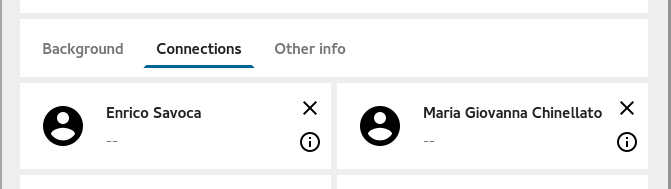
\includegraphics[width=0.7\textwidth]{ConnectionsWidget.png}
\caption{ConnectionsWidget}
\end{figure}

\subsubsection*{OtherInfoWidget}
Mostra tutte le altre informazioni dell'utente, riguardo profilo ed account. In caso sia la scheda del profilo di un contatto o di un risultato della ricerca allora il pulsante di modifica delle informazioni personali viene nascosto. Altrimenti e possibile la modifica tramite la creazione di un oggetto \textbf{EditPersonalInfoDialog} che notifica al parent le modifiche. Le informazioni sull'account (username e tipologia account) non sono modificabili dall'utente.

\subsubsection*{SearchResultWidget}
Alla pressione del pulsante della ricerca nel menu utente (quando il box di ricerca è già aperto) viene fatta la ricerca tra tutti gli utenti del database (escluso l'utente utilizzatore del client) e viene restituita una lista di UserPreviewWidget con gli utenti il quale nome o cognome contiene (ricerca case insensitive) la stringa cercata. In caso di stringa vuota vengono visualizzati tutti gli utenti. Le anteprime sono costruite in base alle informazioni visualizzabili dalla tipologia di account e da tutte è rimosso il pulsante di rimozione dai contatti. La rimozione o l'aggiunta può essere fatta dalla visualizzazione del profilo.

A differenza della scheda dei contatti, i risultati sono disposti in un elenco.

\subsection*{AdminWindow}
Richiama lo stesso design semplice ed intuitivo della classe ClientWindow.

\begin{figure}[!ht]
\centering
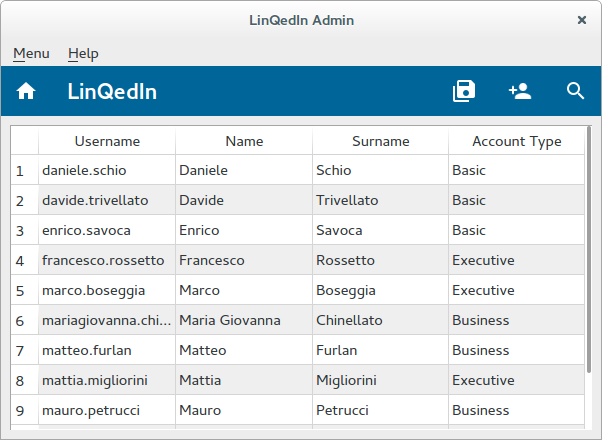
\includegraphics[width=0.6\textwidth]{AdminWindow.png}
\caption{AdminWindow}
\end{figure}

A differenza del client utente, le modifiche possono essere annullate alla chiusura del client. Ad ogni modo il salvataggio è possibile in ogni momento tramite il pulsante presente nel menu. Il menù offre anche la possibilità di aggiunta e ricerca utenti. Il contenuto effettivo della finestra del client è composta da un'istanza di UserListWidget, la quale mostra la lista degli utenti in una tabella.

L'aggiunta di un utente avviene tramite la creazione di un'istanza di \textbf{AddUserDialog}. Allo stesso modo la ricerca avviene tramite un'istanza di \textbf{AdminSearchDialog} ed è possibile selezionare in quali campi tra username, nome e password cercare una determinata stringa.

In caso di selezione di un utente il menu viene sostituito e vengono mostrate le azioni possibili sull'utente selezionato. Queste azioni sono: rimozione utente e cambio tipologia dell'account. Il cambio tipologia avviene tramite un'istanza di \textbf{ChangeUserTypeDialog}.

Contiene due campi dati booleani che indicano se lo stato del database è cambiato e se alla lista degli utenti visualizzata è applicato un filtro.

\subsubsection*{UserListWidget}
La classe UserListWidget funziona come controller (del pattern MVC), dove il model è un'istanza della classe TableModel (derivata da QAbstractTableModel), mentre la view è un'istanza della classe QTableView. Poichè l'inserimento di un nuovo utente avveniva in fondo alla tabella, è stata utilizzata un'istanza della classe MySortFilterProxyModel, derivata da QSortFilterProxyModel. La ridefinizione è stata necessaria anche per permettere la ricerca su più campi.

\subsubsection*{TableModel}
Classe derivata da QAbstractTabelModel. Memorizza il contenuto della tabella in una lista di vettori di oggetti QString. Implementa i metodi \texttt{int rowCount( QModelIndex ) const}, \texttt{int columnCount( QModelIndex ) const}, \texttt{int data( QModelIndex, int ) const} e \texttt{int headerData( QModelIndex, int ) const}, necessari della classe base. Inoltre fornisce un'implementazione per i metodi \texttt{bool insertRows( int, int, QModelIndex )}, \texttt{bool removeRows( int, int, QModelIndex )} e \texttt{bool setData( QModelIndex, QVariant, int )}, per permettere l'inserimento e rimozione di righe dalla tabella.

\subsubsection*{MyProxySortFilterModel}
Se una ricerca viene effettuata con l'utilizzo di QProxySortFilterModel allora questa può essere effettuata solo in una colonna specifica o in tutte (in caso si specifichi indice -1). Per permettere all'amministratore di scegliere su quali campi eseguire la ricerca è stata necessaria la ridefinizione del metodo \texttt{bool filterAcceptsRow( int, QModelIndex ) const}. Con il metodo \texttt{void setFilterKeyColumns( QList<int> = QList<int>() )} si indica quali colonne considerare mentre con \texttt{void addFilterFixedString( int, QString )} si indica quale filtro deve essere applicato ed in quale colonna.

Purtroppo permettere la ricerca anche per tipologia si è rivelata più complicata del previsto e quindi non è stata resa disponibile. Altro problema non risolto è l'aggiornamento degli indici dell'header verticale, in quanto l'utlimo utente inserito avrà sempre indice 1, mentre i risultati di una ricerca hanno come indice quello originale.

\end{document}